\appendix
\chapter{Методы решения задач на построение}

\paragraph{Метод геометрических мест,} известный еще со времен Платона (IV век до нашей эры), состоит в следующем.
Положим, что решение предложенной задачи сводится к нахождению некоторой точки, которая должна удовлетворять известным условиям.
Отбросим из этих условий какое-нибудь одно;
тогда задача сделается неопределенной, то есть ей может удовлетворять бесчисленное множество точек.
Эти точки составят некоторое геометрическое место.
Построим его, если это окажется возможным.

Затем примем во внимание отброшенное нами условие и откинем какое-нибудь другое; 
тогда задача будет снова удовлетворяться бесчисленным множеством точек, которые составят новое геометрическое место.
Построим его, если это возможно.
Искомая точка, удовлетворяя всем условиям, должна лежать на обоих геометрических местах, то есть она должна находиться в их пересечении.

Задача окажется возможной или невозможной, смотря по тому, пересекаются или нет найденные геометрические места; и задача будет иметь столько решений, сколько окажется точек пересечения.

Приведем на этот метод один пример, который вместе с тем покажет нам, как иногда приходится вводить в чертеж вспомогательные построения с целью принять во внимание все данные условия задачи.

\smallskip
\so{Задача}. Построить треугольник по основанию $a$, углу при вершине $A$ и сумме $s$ боковых сторон.

\begin{wrapfigure}{R}{53mm}
\centering
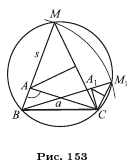
\includegraphics{mppics/ris-153}
\caption{}\label{1931/ris-466}
\end{wrapfigure}

Пусть $ABC$ будет искомый треугольник (рис. \ref{1931/ris-466}).
Чтобы принять во внимание данную сумму боковых сторон, продолжим $BA$ и отложим $BM=s$.
Проведя $MC$, получим вспомогательный треугольник $BMC$.
Если мы построим этот треугольник, то затем легко построим и $\triangle ABC$.
Построение $\triangle  BMC$ сводится к нахождению точки $M$.

Заметив, что $\triangle AMC$ равнобедренный ($AM\z=AC$) и, следовательно, $\angle M = \tfrac\angle A$ (так как $\angle M+\angle C= \angle A$), мы видим, что точка $M$ должна удовлетворять двум условиям: 
1) она удалена от $B$ на расстояние $s$; 
2) из нее данный отрезок $BC$ виден под углом, равным $\tfrac12\angle A$. 

Отбросив второе условие, мы получим бесчисленное множество точек $M$, лежащих на окружности с центром $B$ и радиусом $s$.

Отбросив первое условие, мы получим также бесчисленное множество точек $M$, лежащих на дуге сегмента, построенного на $BC$ и вмещающего угол, равный $\tfrac12\angle A$.

Таким образом, нахождение точки $M$ сводится к построению двух геометрических мест, из которых каждое мы построить умеем.

Задача окажется невозможной, если эти геометрические места не будут иметь общих точек; задача будет иметь одно или два решения, смотря по тому, касаются или же пересекаются эти места (на нашем чертеже получаются два треугольника $ABC$ и $A_1B_1C_1$, удовлетворяющие условиям задачи).

Иногда задача сводится не к определению точки, а к нахождению прямой, удовлетворяющей нескольким условиям. Если отбросим одно из них, то получим бесчисленное множество прямых; при этом может случиться, что эти прямые определяют некоторую линию (например, все они будут касательными к некоторой окружности). Отбросив другое условие и приняв во внимание то, которое было откинуто ранее, мы получим снова бесчисленное множество прямых, которые, быть может, определят некоторую другую линию. Приведем пример.

\so{Задача}. Провести секущую к двум данным окружностям с центами $O$ и $O_1$ так, чтобы части секущей, заключенные внутри окружностей, равнялись соответственно данным длинам $a$ и $a_1$.

Если возьмем только одно условие (например, чтобы часть секущей, лежащая внутри круга О, равнялась а), то получим бесчисленное множество секущих, которые все должны быть одинаково удалены от центра этого круга (так как равные хорды одинаково удалены от центра). Поэтому если в круге О где-нибудь построим хорду, равную а, а затем радиусом, равным расстоянию этой хорды от центра, опишем окружность, концентрическую с О, то все секущие, о которых идет речь, должны касаться этой вспомогательной окружности; подобным образом, приняв во внимание только второе условие, мы увидим, что искомая секущая должна касаться второй вспомогательной окружности, концентрической с О,. Значит, вопрос приводится к построению общей касательной к двум окружностям.
Полезно заметить следующие геометрические места (из которых некоторые были указаны в тексте книги, а доказательство других предоставляем самим учащимся):

1) Геометрическое место точек, одинаково удаленных от двух данных точек А и В, есть перпендикуляр, проведенный к отрезку АВ через его середину (§ 56).
29

2)                                  Геометрическое место точек, одинаково удаленных от сторон угла, есть биссектриса этого угла (§ 56).

3)                                     Геометрическое место точек, удаленных от данной прямой на данное расстояние d, состоит из двух прямых, параллельных данной и расположенных по обе стороны от нее на расстоянии d (§ 92).

4)                                  Геометрическое место точек, из которых данный отрезок прямой виден под данным углом а, состоит из дуг двух сегментов, которые вмещают в себя угол, равный а (§ 130), и расположены по разные стороны данного отрезка.

5)                                  Геометрическое место точек, делящих в данном отношении отрезки параллельных прямых, заключенных между сторонами данного угла, есть прямая, проходящая через вершину угла и какую-нибудь одну из этих точек.

6)                                 Геометрическое место точек, расположенных внутри данного угла и расстояния которых от сторон этого угла находятся в данном отношении т: n, есть прямая, проходящая через вершину угла и какую-нибудь одну из таких точек.

7)                                  Геометрическое место точек, делящих в данном отношении все равные хорды данной окружности, есть окружность, концентрическая с данной.

8)                                  Геометрическое место точек, из которых касательные, проведенные к данной окружности, имеют данную длину, есть окружность, концентрическая с данной.

9)                                  Геометрическое место точек, квадраты расстояний которых от двух данных точек А и В имеют постоянную сумму, есть окружность, центр которой лежит в середине прямой АВ (доказательство основывается на теореме § 168).

10)                                   Геометрическое место точек, квадраты расстояний которых от двух данных точек А и В имеют постоянную разность, есть прямая, перпендикулярная к прямой АВ.

11)                                  Геометрическое место точек, сумма расстояний которых от сторон данного угла постоянна, есть лежащий внутри угла отрезок прямой, отсекающей от угла равнобедренный треугольник. Продолжения этого отрезка (в обе стороны) представляют геометрическое место точек, разность расстояний которых от сторон угла постоянна.

12)                                   Геометрическое место точек, делящих в данном отношении хорды, проведенные из точки А данной окружности, есть окружность, касательная к данной в точке А.
Последнее геометрическое место составляет частный случай следующего более общего (см. § 167-171):

13)                                  Если из данной точки О (черт: 467) к различным точкам А, А" AII, . . . какой-нибудь фигуры F проведем прямые ОА, ОА" OAII, ... и на каждой из них отложим части Оа, Оа", Oal l, . . . такие, что Oa:OA =Oa, :oA, =Oall:OAII = . . . , to геометрическое место точек а, а" al l, ... есть фигура f, подобная фигуре F и одинаково с ней расположенная относительно точки О.
291
Черт, 467
Таким образом, если фигура F есть прямая, то и f есть прямая, параллельная F; если F есть многоугольник, то и f есть многоугольник, подобный F и одинаково с ним расположенный; если F - окружность, то и f - окружность.
Когда пропорциональные части Оа, Оа), Оа)), , .. откладываются на продолжениях линий ОА, ОА) (за точку О), то получается тоже подобная фигура, но расположенная обратно относительно центра подобия О.
К этим геометрическим местам добавим еще следующее: геометрическое место точек, расстояния которых от двух данных точек находятся в данном отношении m:n, есть окружность, когда $m\ne n$, и прямая, когда т = п.
Предварительно покажем, что если $m\ne n$, то на неограниченной прямой MN (черт. 468), проходящей через точки А и В, можно найти две (и только две) точки С и С), принадлежащие указанному геометрическому месту, то есть такие, что СА:СВ = m:п и С)А:С)В = m:п. Чтобы найти такие точки, проведем через А и В две какие-нибудь параллельные между собой прямые и на них отложим AD = m, ВЕ = п и BF = n. Проведя затем DE и DF, получим в пересечении с MN две искомые точки С и С) (последняя точка, конечно, получится только тогда, когда $m\ne n$), так как из подобных треугольников ACD и CBF, а затем из подобных треугольников ADC) и ВЕС) получим пропорции
AC:CB= AD:BF=m:n и
АС) :ВС) =AD:BE = m:n,
Заметив это, допустим, что (при m=n) существует еще какая-нибудь точка Р (черт. 469), удовлетворяющая пропорции
РА:РВ = m:п.
Проведя РС и Р,С), мы должны заключить (176, 178), что первая из этих прямых есть биссектриса угла АРВ, а вторая -биссектриса угла BPQ; вследствие этого угол СРС), составленный из двух половин смежных углов, должен быть прямой, а потому вершина его Р лежит на окружности, описанной на отрезке СС),
292
*F Черт. 468
Черт. 469
как на диаметре. Мы доказали, таким образом, что всякая точка Р, принадлежащая искомому геометрическому месту, лежит на окружности диаметра СС\. Теперь докажем обратное предложение.
Пусть Р (черт. 469) есть произвольная точка этой окружности. Проведя через В прямую EDIIAP, будем иметь следующие пропорции:
\[PA:BD = C_1A:C_1B = m:n\eqno{(1)}\]
и
\[PA:BE=CA:CB=m:n\eqno{(2)}\]
Откуда находим: BD = BE, то есть точка В есть середина прямой DE. Так как угол СРС\ вписанный, опирающийся на диаметр, то он прямой; поэтому ADPE прямоугольный. ВС,Вследствие этого, если середину В гипотенузы DE примем за центр и опишем радиусом BD = ВЕ окружность, то эта окружность пройдет через Р, значит, BD = РВ. Подставив теперь в пропорцию (l) на место BD равную длину РВ, получим: РА:РВ = $m:n$.
Таким образом, мы доказали, что когда т= n, искомое геометрическое место есть окружность, построенная на отрезке СС\ как на диаметре.
Допустим теперь, что т = n. Тогда не будет вовсе точки С\, а точка С окажется лежащей в середине отрезка АВ. Очевидно, что перпендикуляр к АВ, проведенный через эту середину, будет искомым геометрическим местом.

\paragraph{Метод подобия.}
Он состоит в том, что, пользуясь некоторыми данными задачи, строят сначала фигуру, подобную искомой, а затем переходят к последней. Этот метод особенно удобен тогда, когда одна данная величина есть длина, а все прочие или углы, или отношения линий; таковы, например, задачи: построить треугольник по данному углу, стороне и отношению двух других сторон или по двум углам и длине некоторой прямой (высоте, медиане, биссектрисе и т. п.); построить квадрат по данной сумме или разности между диагональю и стороной и т. п.
В этих задачах положение искомой фигуры остается произвольным; но во многих вопросах требуется построить фигуру,
293
А
Черт. 470
положение которой относительно данных точек или линий вполне определенно. При этом может случиться, что, отрешившись от какого-нибудь одного из условий положения и оставив все остальные, мы получим бесчисленное множество фигур, подобных искомой. В таком случае метод подобия может быть употреблен с пользой. Приведем пример. 

\so{Задача}.
В данный угол ABC вписать окружность, которая проходила бы через данную точку М (черт. 470).
Отбросим на время требование, чтобы окружность проходила через точку М. Тогда вопросу удовлетворяет бесчисленное множество окружностей, центры которых лежат на биссектрисе BD. Построим одну из таких окружностей, например ту, центр которой есть о. Возьмем на ней точку т, с х о Д с т в е н н у ю точке М, то есть лежащую на луче подобия МВ, и проведем радиус то. Если теперь построим М О 11 то, то точка О будет центром искомого круга. Действительно, про ведя к стороне АВ перпендикуляры ON и оп, мы получим подобные треугольники МВО и тВо, N ВО и пВо, из которых будем иметь:                                                                                                                                                                                                                                                                                                                                                                                                                                                                                                                                                                                                                                                                                                                                                                    /
МО:то = ВО:Во; NO:no = BO:Bo, откуда
MO:mo = NO:no.
Но то = nо; следовательно, и MO = NO, то есть окружность, описанная из центра О радиусом ОМ, касается стороны АВ; а так как ее центр лежит на биссектрисе угла, то она касается и стороны ВС.
Если за сходственную точку возьмем другую точку т, пересечения луча МВ с окружностью о, то найдем другой центр О, искомого круга. Следовательно, задача допускает два решения.
3. Метод параллельного перенесения. Весьма часто бывает полезно переместить некоторые части данной или искомой фигуры в другое положение, при котором легче обнаружить зависимость между данными элементами и искомыми. Существуют различные приемы такого перемещения. Рассмотрим сначала пара л л е л ь н О е   пер е н е с е н и е   (§ 104).

\so{Задача}. Построить четырехугольник ABCD (черт. 471), зная все его стороны и прямую ЕР, соединяющую середины противоположных сторон.
Чтобы сблизить между собой данные линии, перенесем параллельно самим себе стороны AD и ВС в положения ED, и ЕС,. Тогда прямая DD, будет равна и параллельна АЕ, а прямая сс, равна и параллельна ЕВ; но так как АЕ = ЕВ, то DD, = сс,
294
и DD111 CC1
Вследствие этого треугольники DD1F и CC1F будут равны (так как у них DD1 = CC1, DF=CF и LD1DF = LFCC1);
значит, LD1FD= LCFC1 и потому линия D1FC1 должна быть прямая, то есть фигура ED1FC1 окажется треугольником.
В этом треугольнике известны две стороны (ED1 =AD и ЕС1 =ВС) и медиана EF, проведенная к третьей стороне.
По этим данным легко построить треугольник (если продолжим медиану EF за точку F на длину, равную ей, и полученную точку соединим с D1 и C1, то получим параллелограмм, у которого известны стороны и одна диагональ).
Найдя DED1C1, строим треугольники D1DF и C1CF, а затем и четырехугольник ABCD.
Заметим, что иногда бывает полезно перенести параллельно данному направлению целую фигуру, например окружность (см., например, ниже З{дачу 501) ..

\paragraph{Метод вращения вокруг точки.}
Для уяснения этого особенного вида перенесения приведем следующий пример:

Задача. даны по положению точка С (черт. 472) и две бесконечные прямые Q и Ь. Построить треугольник ABC, одна вершина которого была бы в С, а две другие лежали бы на прямых Q и Ь и который, кроме того, был бы подобен данному треугольнику (не помещенному на чертеже).
Пусть задача решена.
Заметив, что углы искомого треугольника даны, обозначим тот из них, который находится при точке С, буквою. 
Повернем всю фигуру вокруг точки С в направлении, указанном стрелкой, на угол со и найдем положение, которое займет после вращения прямая а. 
Для этого достаточно опустить на Q перпендикуляр CD, а затем повернуть его на угол со в положение CD1 и провести через D1 прямую Ql, перпендикулярную к CD1.
Прямая аl и будет то положение, которое займет после вращения прямая а. 
Так как при вращении все части фигуры повертываются на один и тот же угол, то СА после вращения пойдет по СВ, вследствие этого точка А упадет в A1, то есть в точку пересечения СВ с Ql. 
Так как отношение СА и СВ или, все равно, отношение СА 1 к СВ дано (пусть это будет т: n), то теперь вопрос сведен к тому, чтобы через точку С провести такую прямую СА 1, которая пересекалась бы с прямыми Ь и аl В точках В и А 1, удовлетворяющих пропорции СА 1 : СВ = т: n. 
Чтобы провести такую   прямую,   достаточно   разделить
CD1 в некоторой точке х так, чтобы CD1:Cx = m:n, и через точку деления провести прямую, параллельную al; пересечение этой прямой с Ь определит точку В.

\paragraph{Метод  вращения   вокруг  прямой
(или метод симметрии).} Иногда прием
построения легко обнаруживается, если
перегнем часть чертежа вокруг некоторой
прямой  так,   чтобы  эта  часть  заняла
симметричное положение по другую сто-
ерт.                                                                                                                                                                                                                                                                                                                                                                                                                                                                                                                                                                          рону от этой прямой (§ 36). Приведем
пример.

\so{Задача}. На бесконечной прямой АВ  (черт. 473) найти
точку х, чтобы сумма ее расстояний от данных точек М и N была
наименьшая.
Если, перегнув чертеж вокруг АВ, приведем точку М в симметричное относительно АВ положение M 1 , то расстояние точки М от какой угодно точки прямой АВ сделается равным расстоянию точки М1 от той же точки прямой АВ. Поэтому суммы Mx+xN, МХI +xIN, ... равны соответственно суммам M1x+xN, M1xI +xIN, .. . ; но из последних сумм наименьшая будет та, при которой линия М IxN прямая. Отсюда становится ясным прием построения.
То же самое построение решает и другую задачу: на прямой АВ найти такую точку х, чтобы прямые хМ и xN, проведенные от нее к данным точкам М и N, составяли с АВ равные углы.

\paragraph{Метод обратности.}
Иногда бывает полезно перевернуть, так сказать, задачу, то есть данные условия задачи взять за искомые и наоборот. Приведем пример.

\smallskip

\so{Задача}. В данный треугольник $ABC$ вписать другой треугольник, у которого стороны были бы параллельны сторонам другого данного треугольника $MNP$.

Перевернем вопрос: опишем около $\triangle MNP$ другой $\triangle A_1B_1C_1$, у которого стороны были бы параллельны сторонам $\triangle ABC$ (что, конечно, легко выполнить).
Тогда мы получим фигуру, подобную искомой;
разделив затем какую-нибудь сторону $\triangle  ABC$ на две части, пропорциональные отрезкам сходственной стороны $\triangle A_1B_1C_1$, мы получим одну из вершин искомого треугольника.

\paragraph{Алгебраический метод.} Сущность этого метода, а также и при меры задач, решаемых им, были указаны ранее (§ 205\ 206 и задачи 290—292, 357-364).

\section*{Примеры задач, решаемых методами, указанными в приложениях}

1. Метод геометрических мест

485.                       Построить четырехугольник ABCD, около которого можно было бы описать окружность, зная его стороны АВ и ВС, диагональ АС и угол между диагоналями.

486.                      Построить треугольник по основанию, углу при верш ин е и сумме или разности квадратов двух других сторон (напри мер, основание а, угол при вершине А и сумма квадратов боковых сторон к).

487.                      Около равностороннего треугольника описать квадрат так, чтобы обе фигуры имели общую вершину.

488.                     Найти точку, из которой три отрезка данной прямой АВ, ВС и CD были бы видны под равными углами.

489.                       Внутри треугольника найти такую точку, расстояния которой до сторон треугольника относились бы между собой, как 6:3:2. (См. задачу 272.)

490.                      Найти точку, из которой три данных круга видны под равными углами. (У к а з а н и е. Надо сначала найти геометрическое место точек, из которых два данных круга видны под равными углами.)

491.                      Найти по данной окружности такую точку, чтобы сумма ее расстояний от двух данных прямых была наименьшая.
492.                     Превратить данный треугольник в равновеликий треугольник с данным основанием и с данным углом при вершине.

493.                    В данной окружности провести две хорды данной длины так, чтобы они пересекались под данным углом и одна из них проходила через данную точку.
2. Метод подобия

494.                       Построить треугольник по углу при вершине, высоте и отношению отрезков, на которые основание делится высотой.

495.                    Вписать квадрат: 1) в данный треугольник; 2) в данный сектор; 3) в данный сегмент.

496.                      Через данную точку провести прямую таким образом, чтобы три данные прямые, исходящие из одной точки, отсекали от искомой прямой отрезки, находящиеся в данном отношении.

497.                     Через данную точку А окружности' провести хорду AD, которая пересекалась бы с данной хордой ВС в такой точке Е, чтобы прямые DE и DC находились в данном отношении.

498.                      Провести внутри треугольника прямую, параллельную основанию, так, чтобы эта прямая была средней пропорциональной между отрезками одной боковой стороны.

499.                      Построить равнобедренный треугольник, зная его боковую сторону и сумму высоты с основанием.

500.                      На данной прямой найти такую точку, чтобы расстояния от данной точки и другой данной прямой находились в данном отношении.
297

3. Метод параллельного перенесения

501.                      Между двумя данными окружностями провести данную прямую данной длины а параллельно данной прямой MN. (У к а з а н и е. Надо один круг приблизить к другому, перенеся его параллельно прямой MN на расстояние а.)

502.                      В круге даны две хорды АВ и CD. Найти на окружности такую точку х, чтобы прямые хА и хВ отсекали от хорды CD отрезок, равный данной длине (метод параллельного перенесения и геометрических мест).

503.                        В данном треугольнике ABC найти такие точки: х на стороне АВ и у на стороне ВС, чтобы прямая ху была данной длины и отношение Ах: Су было данное (параллельное перенесение и метод подобия).

504.                      Построить трапецию по одному ее углу, двум диагоналям и средней линии.

505.                      Построить четырехугольник по трем сторонам а, Ь, с и двум углам аир, прилежащим к неизвестной стороне.

506.                     К двум данным кругам провести общую секущую, параллельную данной прямой, так, чтобы сумма или разность хорд, определяемых точками пересечений, была равна данной длине.

507.                        С корабля видны два маяка, положения которых на карте известны под данным углом. Когда корабль прошел известную длину в данном направлении, те же самые маяки видны под другим данным углом. Определить на карте место корабля. (Геометрическое место и параллельное перенесение.)

4. Метод вращения вокруг точки

508.                     Построить треугольник, подобный данному треугольнику, так, чтобы одна его вершина лежала в данной точке А, а две другие вершины находились на данных окружностях О и 01 (одна на О, другая на 01)'

509.                     Дан круг и вне его две точки А и В; провести к кругу касательную так, чтобы расстояния точки А до этой касательной и до перпендикуляра, опущенного из В на касательную, были в данном отношении. (У к а з а н и е. Надо повернуть вокруг точки А на 900 прямоугольный треугольник, у которого гипотенуза есть АВ, а один катет - расстояние точки А до перпендикуляра, опущенного на касательную из точки В.
Эту же задачу можно решить при помощи одновременного пользования методом подобия и методом геометрических мет.)

510.                     Построить треугольник, стороны которого были бы пропорциональны числам 3, 4 и 5 и вершины которого лежали бы на трех данных параллельных прямых.
5. Метод вращения вокруг прямой

511.                    Построить по четырем сторонам четырехугольник ABCD, зная, что его диагональ АС делит угол А пополам.

512.                       Конечная прямая АВ пересечена в точке С прямой MN. Найти на MN такую точку, из которой отрезки АС и ВС видны под равными углами (эту задачу можно также решить методом геометрических мест).

513.                       Построить квадрат, две противоположные вершины которого находились бы на двух данных окружностях, а две другие - на данной прямой, расположенной между окружностями.

514.                      На прямоугольном бильярде дано положение двух шаров А и В. В каком направлении надо толкнуть шар А, чтобы он, отразившись последовательно от всех четырех бортов, ударил затем шар В?

515.                     Дан угол и внутри его точка. Построить треугольник наименьшего периметра такой, чтобы одна его вершина лежала в данной точке, а две другие на сторонах угла.

516.                     Решить методом симметрии задачу. которая в тексте была решена методом подобия: в данный угол вписать окружность, которая проходила бы через точку, данную внутри угла.

